\documentclass[a4paper,english, 11pt]{article}


\usepackage[utf8]{inputenc}
\usepackage[T1]{fontenc}
\usepackage{lmodern} 
\usepackage[table]{xcolor}
\usepackage{parskip} 
\usepackage{amssymb,amsthm,framed}  
\usepackage[]{amsmath} 
\usepackage[hang,small,bf]{caption}
\usepackage{siunitx} 
\usepackage{bm}
\usepackage{url}  
\usepackage{multirow} 
\usepackage[hidelinks]{hyperref}
\usepackage[a4paper,inner=2.5cm,outer=2.5cm,top=2.5cm,bottom=2.5cm,pdftex]{geometry} 
\usepackage{array}
\usepackage{ragged2e}
\newcolumntype{P}[1]{>{\RaggedRight\hspace{0pt}}p{#1}}

\sisetup{product-units=single}

%  
\usepackage{listings}
\lstset{language=bash}
\lstset{basicstyle=\ttfamily,
  numbers=left,
  showstringspaces=false,
  commentstyle=\color{red},
  keywordstyle=\color{black},
  breaklines=true,
  belowskip=0.5em
}


\usepackage{accsupp}    
\lstset {
    numberstyle=\noncopynumber,
    columns=flexible,
}

\newcommand{\noncopynumber}[1]{
    \BeginAccSupp{method=escape,ActualText={}}
    #1
    \EndAccSupp{}
}


\usepackage{graphicx}     

\usepackage{enumitem}      
\graphicspath{{../Images/}} 
 
\hyphenpenalty=5000
\tolerance=1000
\title{Draft: The Nansen Legacy labeling manual}
\date{\today\\v0.1}
\author{Pål Ellingsen (\url{pale@unis.no})}

\begin{document}
\maketitle
\tableofcontents
\section{Introduction} % (fold) {{{
\label{sec:Introduction}

The Nansen Legacy project is aimed at generating samples, data and science relevant during the project and after its conclusion. Additionally it is a collaboration between major marine institutions in Norway. To accommodate the tracking of samples between from ship to land and  between institutions it was decided to use a unified labeling system. To secure that the project data and metadata follows the FAIR (Findable, Accessible, Interoperable, Reproducible) principle for data management within the project, a first step is to ensure that the collected samples are findable and that relevant metadata are logged
along with the sample collection. The metadata needs to be logged in a standardized manner and will be
made accessible through a search interphase as soon as possible after the cruises.  This manual details how to label samples, log the metadata and how to find information about logged samples in the SIOS database.  

% section Introduction (end) }}}


\subsection{Hierarchy} % (fold) {{{
\label{sub:Hirarcy}

One of the backbones of the sample log is the use of parent IDs. A parent ID is the ID of the gear cast or sample which a sample or sub-sample comes from, see figure~\ref{fig:parent_uuid}. By registering the parent, it is possible to keep track of which samples belong together, and any number of levels of sub-samples. Additionally it reduces the amount of information that needs to be registered on a sample, as information like for example position, bottom depth, date and time can be inherited from the parent. 
\begin{figure}[hp]
    \centering
    \includegraphics[width=1\textwidth]{Labeling.pdf}
    \caption{\label{fig:parent_uuid}
       Examples of how event id and parent id works for two different gear types. These should be transferable to other gear types.
    }
\end{figure}
% subsection Hirarcy (end) }}}

\section{Labeling samples} % (fold) {{{
\label{sec:Labeling samples}



In order to distinguish samples, samples in the project are assigned a unique id, in the form of a universally unique identifier (UUID). Details about it can be found in subsection~\ref{sub:UUID}. For physical samples this UUID is encoded in the form of a 2D barcode, specifically a Data Matrix (DM) code, details in subsection~\ref{sub:DM}. An example of such a code can be seen in figure~\ref{fig:data_matrix}. The code is then printed, together with descriptive text, onto a label which is stuck on the sample or its container.

\begin{figure}[htb]
    \centering
    \includegraphics[width=0.1\textwidth]{Data_matrix.png}
    \caption{\label{fig:data_matrix}
        Example Data Matrix code containing an UUID.
    }
\end{figure}

\subsection{Procedure for physical samples} % (fold) {{{
\label{sub:Procedure for physical samples}


The interface for printing labels is available through a webpage on the research ship. Details of this is given by the cruise leader.

\begin{enumerate}
    \item Choose label size.
    \item Write information which is to be printed together with the label into the printing page. This should include the date and information about what the sample is.
    \item Print the label.  
\end{enumerate}
The following steps can be done in any order depending on what is easiest:
\begin{enumerate}
\setcounter{enumi}{3}
    \item Stick the label on the sample
    \item Register data about the sample in the spreadsheet, see section~\ref{sub:spreadsheet_reg}.
\end{enumerate}

% subsection Procedure for physical samples (end) }}}

\subsection{Procedure for virtual samples} % (fold) {{{
\label{sub:Procedure for virtual samples}

Examples of virtual sample are: gear casts, Multicores, Multinets and Ice cores that have been split/melted. Since these have no physical place for a label to go, the procedure of logging them involves either printing a sheet of paper with the codes or just assigning them a UUID without any Data Matrix code. Which approach is the best depends on the circumstance. If the UUID is going to be used by more than one scientist, for example in the case of Niskin bottles, it is often easier to print an A4 page with the codes. Below follows two different procedures depending on what is chosen:

\subsubsection{A4 page of codes} % (fold) {{{
\label{ssub:A4_page}

Go to the ''Gear UUID generator'' page on the printing overview (address distributed on the cruise). 
On this page you specify the name of the gear ''Gear Name'' (CTD, Multinet, Multicorer), the type of container ''Sample Name'' (Niskin, core, net), number of samples in on gear cast ''Number of samples'' and number of gear casts expected ''Number of pages'' (this is only to save having to come to this page for every cast). 

By pressing ''Make PDF'' a PDF is generated and can be printed on an normal printer. The A4 page printed should be marked with information identifying which gear cast this is for. Then all the containers need to registered in the same way physical samples are, see subsection~\ref{sub:spreadsheet_reg}.

\textbf{Note: It is very important that one person is responsible for registering the containers, as without them samples will be without parents and untraceable.}

If copies are needed for several scientists to work on the same containers, the A4 page can be copied on a copier. 

% subsubsection A4_page (end) }}}

\subsubsection{Only UUID} % (fold) {{{
\label{ssub:Only_UUID}

When only the UUID is needed, one can be generated through the ''UUID generator'' on the printing overview. Pick one of them and continue the registration as in subsection~\ref{sub:spreadsheet_reg}. Remember to ''Get new UUID'' for every time you leave the page in order to ensure that a UUID is used twice.  

% subsubsection Only_UUID (end) }}}
% subsection Procedure for virtual samples (end) }}}


\subsection{Generation of sample log spreadsheet} % (fold) {{{
\label{sub:Sample_log_spreadsheet_generation}

In order to log the samples labeled on a cruise, a standardised spreadsheet is used. The spreadsheet is based on Darwin Core. A generator for the spreadsheet can be found on the SIOS page (or on the ship), specifically at \url{https://www.sios-svalbard.org/cgi-bin/darwinsheet/?setup=aen}. When loading the page, certain parameters are already ticked, these are mandatory and should not be removed. 
The procedure is then to select the wanted columns, this should be done with some cooperation within research groups, as to make sure wanted information is registered. If a column is forgotten, a new sheet can be generated and the column copied into an existing spreadsheet.

When working with the spreadsheet the order of columns can be changed, but it is important to move the whole column as the third row contains the key used by the data manager to read the log into the database. 

It is possible to add additional columns to the spreadsheet that will not end up in the sample log, as any column with an empty third row is ignored. The same goes with rows with an empty event id. 


% subsection   (end) }}}

\subsection{Sample logging} % (fold) {{{
\label{sub:spreadsheet_reg}


The samples taken during a cruise need to be logged in a standardised spreadsheet, see subsection~\ref{sub:Sample_log_spreadsheet_generation} for how to make one. Logging of samples should be done continuously during the cruise. 

When logging the sample you will need its id, for physical samples this id goes in the Sample ID field and should be entered by scanning the Data Matrix code on the sample label. Then its parent, see subsection~\ref{sub:Hirarcy}, needs to be registered, what the parent is depends on what type of sample it is, see figure~\ref{fig:parent_uuid} for some examples. Having registered these two, the rest of the columns in the spreadsheet needs to be filled out. Every column has an explanation of what is expected in the given field. 

To check a sample log there is a spreadsheet checker available on the ship and on the SIOS page ????.
Note that the sheet named ''Metadata'' needs to be filled out before running the checker.


% subsection Sample log spreadsheet logging (end) }}}
\section{Label types} % (fold) {{{
\label{sub:Labels}

When selecting labels there are several considerations to be taken into account. Important considerations are which conditions will the labels be subject to and what type of container are they going on.

In the Nansen Legacy several different labels are available and can be printed on the Zebra label printers on the ship. Table~\ref{tab:labels} contains an overview of them and should be used to choose the appropriate one.

\begin{table}[htb]
    \rowcolors{3}{cyan!10}{white}
    \caption{\label{tab:lables}An overview of different labels and their properties. All labels are waterproof and can withstand most laboratory chemicals}
    \begin{tabular}{l|P{3cm}lP{4cm}P{4cm}}
        \hline
        \textbf{Label} & \textbf{Size} & \textbf{Temp. range} & \textbf{Amount of text} & \textbf{Notes} \\ \hline
        Small& \SI{10}{\mm} diameter & \SIrange{-80}{135}{\celsius} & No text, only DM & Problems sticking on certain plastic bags in \SI{-20}{\celsius}\\
        Medium& \SI{19 x 25}{\mm}, fits Eppendorf \SI{2}{\ml} tubes & \SIrange{}{}{\celsius} & 4 lines of 18 characters each & Problems sticking on certain plastic bags in \SI{-20}{\celsius}. \\
        Large& \SI{25 x 51}{\mm} & \SIrange{-80}{135}{\celsius} & 4 lines of 20 characters each, one with 36 characters. & Problems sticking on certain plastic bags in  \SI{-20}{\celsius}.\\
        \hline
    \end{tabular}
\end{table}



% section Marking samples (end) }}}
\appendix

\section{Technical details} % (fold) {{{
\label{sec:Technical details}

\subsection{UUID} % (fold) {{{
\label{sub:UUID}

\subsubsection{Generation} % (fold) {{{
\label{ssub:Generation}

The reason for using UUID (universally unique identifier) to mark samples is that, given a good seed, the generation of UUIDs (with for example UUID1) ensures that the code is unique (the probability of collision is on the order of $ 2\times10^{-18}$). UUID1 contains the time and information about the computer generating it. It is a good code to use in the Nansen Legacy as the first 8 characters are sequential (it is time) and can be printed in clear text on the label to help with finding samples. UUID generation is implemented in most languages, and is easily done in for instance Python by importing the built in library \emph{uuid}. 

% subsection Generation (end) }}}

\subsubsection{Data Matrix} % (fold) {{{
\label{ssub:DM}
Samples are identified by UUIDs in the for of hex numbers, example \emph{388613ee-1a67-11e9-b5cc-a0481c9e7d26}. As these contain 36 characters, it is impractical to manually type these, therefore they are printed in the form of  Data Matrix (DM) codes following the ECC 200 standard. To fit the UUID the code is of size  $22\times22$, see figure~\ref{fig:data_matrix}. These DMs can be printed in different sizes and read by 2d barcode readers, webcameras and mobile phones. 


% subsection Data Matrix (end) }}}

\subsection{Printer} % (fold) {{{
\label{sub:Printer}
To ensure that the labels can be printed in the field and that the marking stays on, thermal transfer printers are used. One printer is available for each label size. In addition to printing the Data Matrix code, these printers are able to add information from each scientist in human readable format (text), helping to identify the sample without the need to scan it each time.

The chosen printer is a \emph{Zebra GX430t} printer. It was chosen as it puts few limitations on the labels used, and it can be printed to both from software and custom written Python software in the form of a web page. To specify what is printed ZPL codes are used. These support Data Matrix codes following ECC 200.

% subsection Printer (end) }}}

In operation the printer uses ribbon, which needs to periodically be changed, though this is not a large running cost.

\subsection{Scanner} % (fold) {{{
\label{sub:Scanner}

Data Matrix codes can be read with a smartphone or webcamera, though this is not as fast as a dedicated scanner, but it is useful for scanning samples at home institutions. On the ship there are USB scanners available which should be used to insert the UUID codes in the spreadsheet. They work like keyboards, place the cursor in the desired cell and press the scan button on the scanner.

There are two different types of scanners, the \emph{Opticon OPI-3601} and the \emph{Datalogic PowerScan PD9530-DPM}. Most scientists like the \emph{Opticon} the best, but for environments with a lot of water the more expensive and waterproof \emph{Datalogic} is recommended.
% subsection Scanner (end) }}}

% section Technical details (end) }}}

\section{Costs} % (fold) {{{
\label{sec:Costs}

The cost of the purposed solutions are shown in table~\ref{tab:costs}.
\begin{table}[htb]
    \rowcolors{3}{cyan!10}{white}
    \caption{\label{tab:costs}The unit costs}
    \begin{tabular}{lllrr}
        \hline
        \textbf{Item} & \textbf{Need} & \textbf{Unit size} & \textbf{Unit price} & \textbf{Total price} \\ \hline
        CILS Eppendorf label    & 5 000     & Per label  (5 000)    & 2.16 NOK  & 10 800 NOK\\ 
        CILS Eppendorf label    & 20 000    & Per label  (20 000)   & 1.33 NOK  & 26 661 NOK\\ 
        CILS Larger label       & 5 000     & Per label  (5 000)    & 2.14 NOK  & 10 675 NOK\\ 
        CILS Larger label       & 20 000    & Per label  (20 000)   & 1.55 NOK  & 31 107 NOK\\ 
        Zebra GX430t            & 3         & Per unit              & 4950 NOK  & 14 850 NOK\\ 
        Zebra 2300 print ribbon & 3         & $12\times74$~m         & 320 NOK   & 960 NOK\\ 
        Datalogic PD9530-DPM    & 3         & Per unit              & 6478 NOK  & 19 434 NOK\\ 
        \hline
    \end{tabular}
\end{table}


Based the costs presented in the table and the initial needs (20 000 Eppendorf and 5 000 larger labels) the total cost comes to about \textbf{73 000 NOK}.
% section Costs (end) }}}

\end{document} 
